O diâmetro mínimo do tambor e das polias é dado pela equação:

\begin{equation}
  D = H_1 \cdot H_2 \cdot d_c
  \label{eq:diametro_minimo_do_tambor}
\end{equation}

Onde:

\begin{itemize}[leftmargin=1.25cm]
  \item $D$: diâmetro mínimo do tambor e das polias em $\si{\milli\meter}$.
  \item $H_1$: coeficiente segundo a norma NBR 8400 \cite{nbr8400}.
  \item $H_2$: coeficiente segundo a norma NBR 8400 \cite{nbr8400}.
  \item $d_c$: diâmetro do cabo em $\si{\milli\meter}$ (Tabela \ref{tab:propriedades_cabo_adotado}).
\end{itemize}

\vspace{1em}

O coeficiente $H_1$ e $H_2$ foram obtidos na tabela 28 e 29 da NBR 8400 \cite{nbr8400}:

\begin{figure}[H]
  \centering
  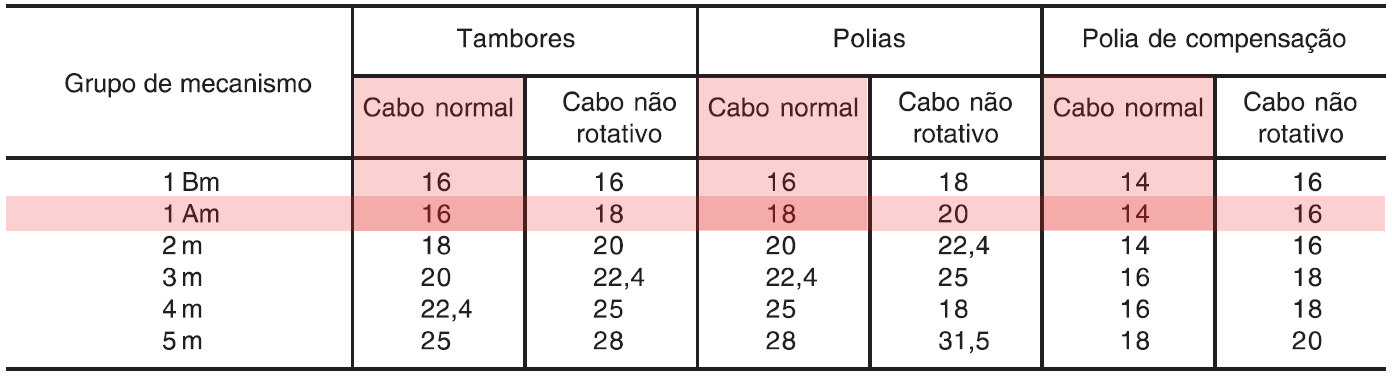
\includegraphics[width=0.7\textwidth]{content/sections/03_sistema_de_elevacao/sections/06_diametro_do_tambor_e_das_polias/images/coeficiente_h1.png}
  \caption{Valores de $H_1$ \cite[p.~34]{nbr8400}}
  \label{fig:coeficiente_h1}
\end{figure}

\begin{figure}[H]
  \centering
  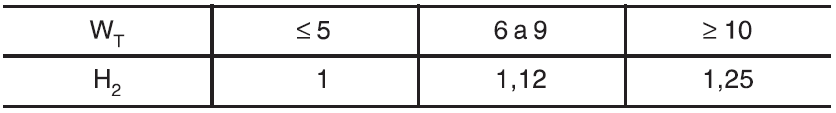
\includegraphics[width=0.5\textwidth]{content/sections/03_sistema_de_elevacao/sections/06_diametro_do_tambor_e_das_polias/images/coeficiente_h2.png}
  \caption{Valores de $H_2$ \cite[p.~34]{nbr8400}}
  \label{fig:coeficiente_h2}
\end{figure}

Segundo a norma NBR 8400 \cite{nbr8400}, para tambores e polias de compensação, $H_2 = 1$. Para polias de passagem, $H_2$ depende de $W_T$, obtido a partir do número de polias e do número de inversões no sentido de enrolamento do cabo. A seguir, apresenta-se um exemplo de $W_T$ para um moitão de quatro cabos, conforme a NBR 8400 \cite{nbr8400}.

\begin{figure}[H]
  \centering
  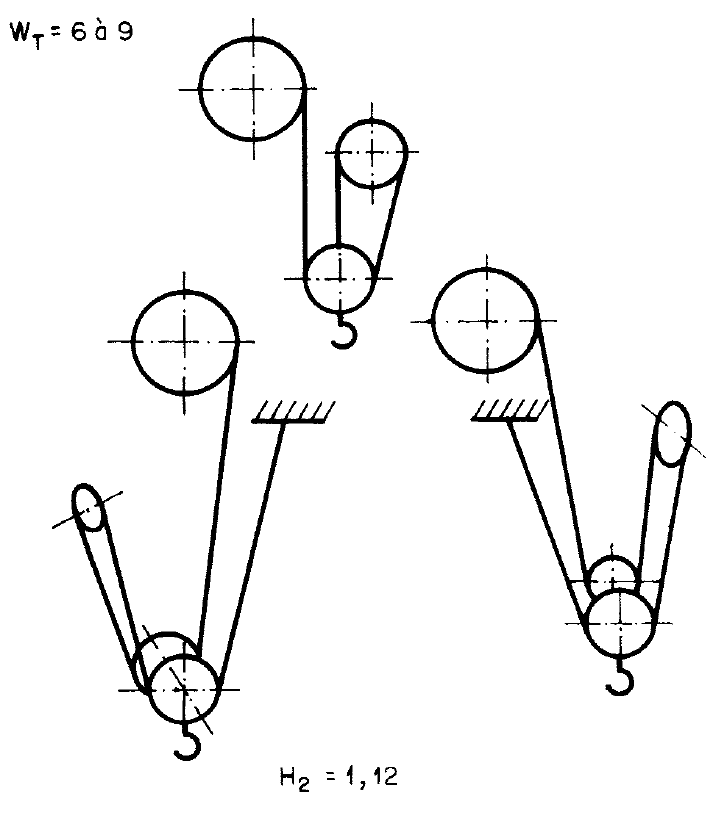
\includegraphics[width=0.5\textwidth]{content/sections/03_sistema_de_elevacao/sections/06_diametro_do_tambor_e_das_polias/images/moitao_wt.png}
  \caption{Exemplo de $W_T$ para um moitão de 4 cabos \cite[p.~35]{nbr8400}}
  \label{fig:moitao_wt}
\end{figure}

Para o grupo de mecanismo 1AM e cabo normal, adotou-se $W_T =$ 6 a 9.
Com isso, obtiveram-se os seguintes valores para os coeficientes $H_1$ e $H_2$:

\begin{table}[H]
  \centering
  \caption{Coeficientes $H_1$ e $H_2$ obtidos segundo a NBR 8400}
  \begin{tabularx}{\textwidth}{>{\centering\arraybackslash}X>{\centering\arraybackslash}X>{\centering\arraybackslash}X}
    \toprule
    Componente           & $H_1$ & $H_2$    \\
    \midrule
    Tambor               & $16$  & $1$      \\
    Polia                & $18$  & $\num{1.12}$ \\
    Polia de Compensação & $14$  & $1$      \\
    \bottomrule
  \end{tabularx}
\end{table}

Substituindo os valores na equação \eqref{eq:diametro_minimo_do_tambor}:

\begin{align*}
  D_t & = 16 \cdot 1 \cdot 19            \\
  D_t & = \boxed{\SI{304}{\milli\meter}}
\end{align*}

\begin{align*}
  d_p & = 18 \cdot \num{1.12} \cdot 19            \\
  d_p & = \boxed{\SI{383.04}{\milli\meter}}
\end{align*}

\begin{align*}
  d_{p_{\text{compensação}}} & = 14 \cdot 1 \cdot 19            \\
  d_{p_{\text{compensação}}} & = \boxed{\SI{266}{\milli\meter}}
\end{align*}

Como os diâmetros de tambores são usualmente padronizados em incrementos de \SI{50}{\milli\meter}, adotou-se o diâmetro nominal de \boxed{\SI{350}{\milli\meter}}.

Com base no catálogo de polias da BOHMER, adotaram-se polias com diâmetro de \SI{500}{\milli\meter}, para cabos de \SI{20}{\milli\meter}. O tipo selecionado foi o de polia para moitão inferior com duas roldanas, conforme a DIN 15408. Como o catálogo não informa o peso unitário, adotou-se \SI{80}{\kilo\gram} por polia. As polias selecionadas são apresentadas a seguir:

\begin{figure}[H]
  \centering
  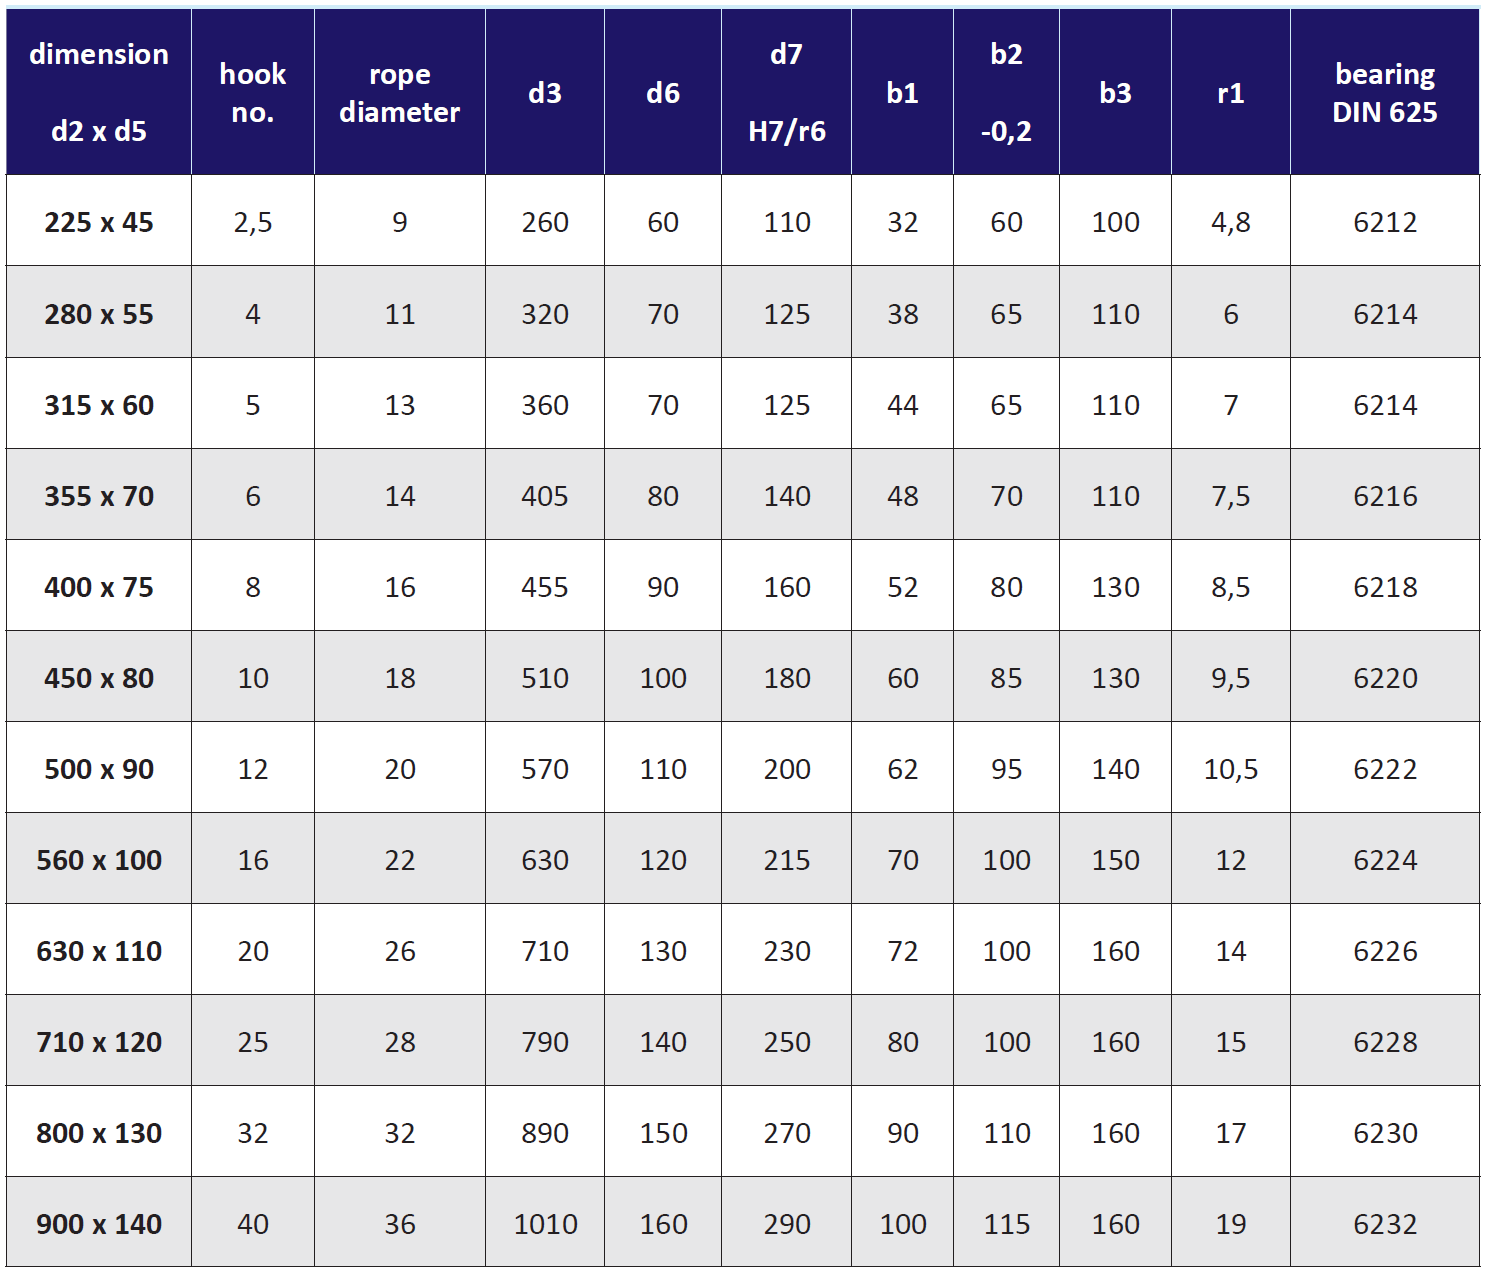
\includegraphics[width=0.6\textwidth]{content/sections/03_sistema_de_elevacao/sections/06_diametro_do_tambor_e_das_polias/images/polias_bohmer.png}
  \caption{Polias do catálogo \cite[p.~3]{bohmer_polias}}
  \label{fig:polias_bohmer}
\end{figure}
